\documentclass[12pt, twoside]{article}
\documentclass[12pt, twoside]{article}
\usepackage[letterpaper, margin=1in, headsep=0.2in]{geometry}
\setlength{\headheight}{0.6in}
%\usepackage[english]{babel}
\usepackage[utf8]{inputenc}
\usepackage{microtype}
\usepackage{amsmath}
\usepackage{amssymb}
%\usepackage{amsfonts}
\usepackage{siunitx} %units in math. eg 20\milli\meter
\usepackage{yhmath} % for arcs, overparenth command
\usepackage{tikz} %graphics
\usetikzlibrary{quotes, angles}
\usepackage{graphicx} %consider setting \graphicspath{{images/}}
\usepackage{parskip} %no paragraph indent
\usepackage{enumitem}
\usepackage{multicol}
\usepackage{venndiagram}

\usepackage{fancyhdr}
\pagestyle{fancy}
\fancyhf{}
\renewcommand{\headrulewidth}{0pt} % disable the underline of the header
\raggedbottom
\hfuzz=2mm %suppresses overfull box warnings

\usepackage{hyperref}
\usepackage{float}

\title{Algebra 2}
\author{Chris Huson}
\date{June 2024}

\fancyhead[LE]{\thepage}
\fancyhead[RO]{\thepage \\ Name: \hspace{1.5cm} \,\\}
\fancyhead[LO]{BECA/Huson/Algebra 2: Regents Preparation \\* 12 June 2024}

\begin{document}
\subsubsection*{Prep \#28 Polynomial functions}
\begin{enumerate}
\item Given the function $f(x)=x^3-3x^2+4$. Graph $f$ on the axes below.
    \begin{enumerate}[itemsep=1.5cm]
        \item Write down the zeros of the function.
        \item Write an equation to represent $f(x)$ in factored form.
        \item Which factor has a multiplicity of 2?
        \item Find the average rate of change of the function over the interval $0 \leq x \leq 2$.
    \end{enumerate} \vspace{2cm}
    \begin{center}
        \begin{tikzpicture}[scale=1]
        \draw[gray,thin] (-6,-4) grid[xstep=1,ystep=1] (6,6);
        \draw [thick,->] (-6,0)--(6.3,0) node [above] {$x$};
        \draw [thick,->] (0,-4)--(0,6.5) node [above] {$y$};
        \foreach \x in {-6,-4,-2,2,4,...,6}
            \draw (\x,5pt) -- (\x,-5pt) node[below] {$\x$};
        \foreach \y in {-4,-2,2,4,...,6}
            \draw (2pt,\y cm)--(-2pt,\y cm) node[left]{$\y$};
        %\draw [thick,->, domain=-3:3.1,smooth,samples=100] plot (\x,{2^\x});
        %\draw [thick,->, domain=0.125:8.3,smooth,samples=100] plot (\x,{log2(\x)});
            \end{tikzpicture}
        \end{center}

\newpage
\item Tony is evaluating his retirement savings. He currently has \$318,000 in his account, which earns an interest rate of 7\% compounded annually. He wants to determine how much he will have in the account in the future, even if he makes no additional contributions to the account.
    \begin{enumerate}
        \item Write a function, \( A(t) \), to represent the amount of money that will be in his account in \( t \) years. \vspace{1.cm}
        \item Graph \( A(t) \) where \( 0 \leq t \leq 20 \) on the set of axes below.
        \item Find how many years it would take for Tony's account to reach \$1,000,000, to the \emph{nearest year}. \vspace{1.5cm}
    \end{enumerate}
    \begin{center}
    \begin{tikzpicture}[scale=0.65]
        \draw[thin,gray] (0,0) grid (20,20);
        \draw[thick,->] (0,0) -- (20.5,0) node[below] {$x$};
        \draw[thick,->] (0,0) -- (0,20.5) node[above] {$A(x)$};
    \end{tikzpicture}
    \end{center}

    
\end{enumerate}
\end{document}